%
% !TeX root =./main.tex
% !TeX spellcheck = en_US
\subsection{Matrix Representation of the Road Network}

For now, we consider the \textit{higher level road network} in Carinthia,
i.e., \textit{A}, \textit{S}, \textit{L}, \textit{B}, in form of a matrix.
The vertices of the matrix are the crossing points of the roads, while
the road section connecting those points form the edges of the matrix.
For each edge, we have the distance between the vertices and the length of the bridges along the segment and the capacity constraints (and the lowest encountered bridge capacity) for each edge.
This way, we can answer various questions concerning transports between those vertices.


\begin{figure}[!ht]
 \centering
  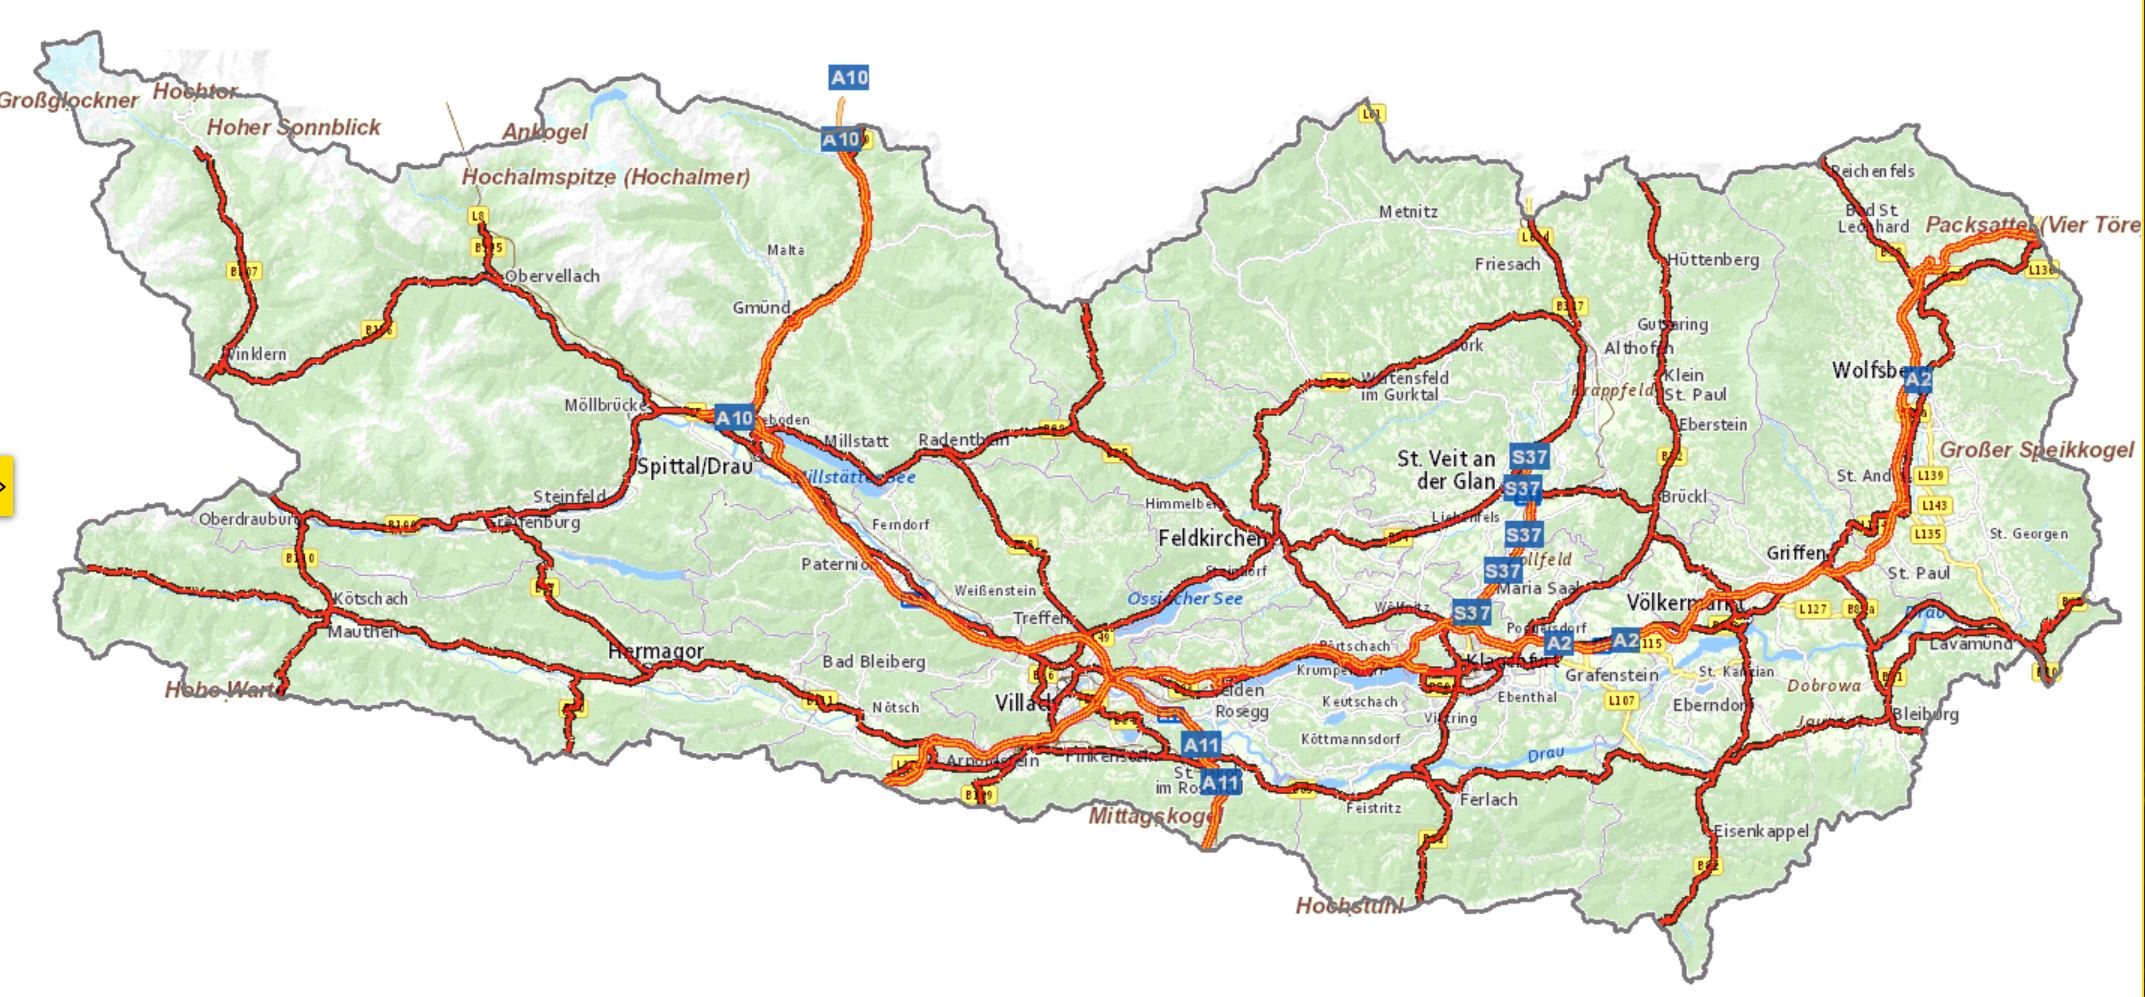
\includegraphics[width=0.9\textwidth]{map.jpg}
  \caption{Overview of the higher level road network in Carinthia.}
  \label{fig:higher level}
\end{figure}
